% figure check fixture (#1054): paper-twin-loop.tex's connector defects,
% cut down. The `reading` arrow stops at the twin's height but beside its
% box (c7), and the `relay` tag is set with no gap from its line (c2).
\usetikzlibrary{positioning}%
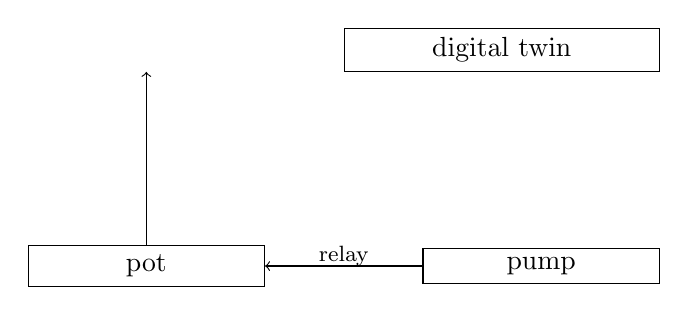
\begin{tikzpicture}[lbl/.style={font=\footnotesize,fill=white,inner sep=0pt}]
  \node[draw,minimum width=30mm] (pot) {pot};
  \node[draw,minimum width=30mm,right=20mm of pot] (pump) {pump};
  \node[draw,minimum width=40mm,above right=22mm and 10mm of pot] (twin) {digital twin};
  \draw[->] (pot.north) -- (pot.north |- twin.south);
  \draw[->] (pump) -- (pot) node[lbl,pos=0.5,above] {relay};
\end{tikzpicture}%
